% Compilar a .pdf con LaTeX (pdflatex)
% Es necesario instalar Beamer (paquete latex-beamer en Debian)
%


\documentclass{beamer}
\usetheme{Warsaw}
\beamertemplatenavigationsymbolsempty
\setbeamertemplate{headline}{}
\useoutertheme{infolines}
%\usebackgroundtemplate{
\includegraphics[width=\paperwidth]{format/libresoft-bg-soft.png}}
\usepackage[spanish]{babel}
\usepackage[utf8]{inputenc}
\usepackage{graphics}
\usepackage{amssymb} % Simbolos matematicos
\usepackage{multicol}

%\definecolor{libresoftgreen}{RGB}{162,190,43}
%\definecolor{libresoftblue}{RGB}{0,98,143}

%\setbeamercolor{titlelike}{bg=libresoftgreen}

%% Metadatos del PDF.
\hypersetup{
  pdftitle={Frikiminutos 2016 (enero--abril, serie B)},
  pdfauthor={Jesús M. González Barahona, Gregorio Robles},
  pdfcreator={GSyC, Universidad Rey Juan Carlos},
  pdfproducer=PDFLaTeX,
  pdfsubject={},
}
%%

%%%%%%%%%%%%%%%%%%%%%%%%%%%%%%%%%%%%%%%%%%%%%%%%%%%%%%%%%%%%%%%%
%%%%%%%%%%%%%%%%%%%%%%%%%%%%%%%%%%%%%%%%%%%%%%%%%%%%%%%%%%%%%%%%
% include-only                                                 %
%%%%%%%%%%%%%%%%%%%%%%%%%%%%%%%%%%%%%%%%%%%%%%%%%%%%%%%%%%%%%%%%
%%%%%%%%%%%%%%%%%%%%%%%%%%%%%%%%%%%%%%%%%%%%%%%%%%%%%%%%%%%%%%%%
%\includeonly{gutenberg}

\AtBeginSection[]
{
\begin{frame}<beamer>
\begin{center}
{\Huge \insertsection}
\end{center}
\end{frame}
}

\begin{document}

\title{Frikiminutos 2016 (enero--abril), serie B}
\subtitle{ETSIT -- URJC}
\author{Jesús M. González Barahona, Gregorio Robles Martínez}
\institute{\url{http://gsyc.es/~jgb}~~~\url{http://gsyc.es/~grex/} \\
GSyC, Universidad Rey Juan Carlos}

%\date{Enero 2015}

\frame{
\maketitle
\begin{center}

\includegraphics[width=6cm]{../format/gsyc-urjc}
\end{center}
}


% Si el titulo o el autor se quieren acortar para los pies de página
% se pueden redefinir aquí:
%\title{Titulo corto}
%\author{Autores abreviado}


%% LICENCIA DE REDISTRIBUCION DE LAS TRANSPAS
\frame{
~
\vspace{3cm}

\begin{flushright}

\includegraphics[width=2.2cm]{figs/by-sa}

\begin{footnotesize}
\copyright 2015-2016 Gregorio Robles, Jesús M. González Barahona. \\

Algunos derechos reservados. Este artículo se distribuye bajo
la licencia ``Reconocimiento-CompartirIgual 3.0 España'' de Creative Commons,
disponible en \\
{\small \url{http://creativecommons.org/licenses/by-sa/3.0/es/deed.es}}

Este documento (o uno muy similar) está disponible en \\
\url{http://cursosweb.github.io} \\
\end{footnotesize}
\end{flushright}
}
%%

\begin{frame}
\begin{multicols}{2}
\tableofcontents
\end{multicols}
\end{frame}


%%%%%%%%%%%%%%%%%%%%%%%%%%%%%%%%%%%%%%%%%%%%%%%%%%%%%%%%%%%%%%%%
%%%%%%%%%%%%%%%%%%%%%%%%%%%%%%%%%%%%%%%%%%%%%%%%%%%%%%%%%%%%%%%%
% lista de temas                                               %
%%%%%%%%%%%%%%%%%%%%%%%%%%%%%%%%%%%%%%%%%%%%%%%%%%%%%%%%%%%%%%%%
%%%%%%%%%%%%%%%%%%%%%%%%%%%%%%%%%%%%%%%%%%%%%%%%%%%%%%%%%%%%%%%%
\include{panopticlick} % jgb
\section{Trabajo top}

%-----------------------    ---------------------------------

\begin{frame}
\frametitle{¿Qué es un trabajo \emph{bueno}?}

\begin{itemize}
   \item Un trabajo que te permita ser creativo
   \item Un trabajo donde trabajes con últimas tecnologías
   \item Un trabajo donde puedas ascender sin dejar de ser ingeniero
   \item Un trabajo donde te paguen bien (y otros beneficios)
\end{itemize}

Hay muchas empresas donde buscan este tipo de perfil: Google, Apple, Facebook,
Microsoft, Yahoo!, Amazon...

\end{frame}

%-----------------------    ---------------------------------

\begin{frame}
\frametitle{Salarios en las compañías top}

\begin{center}
  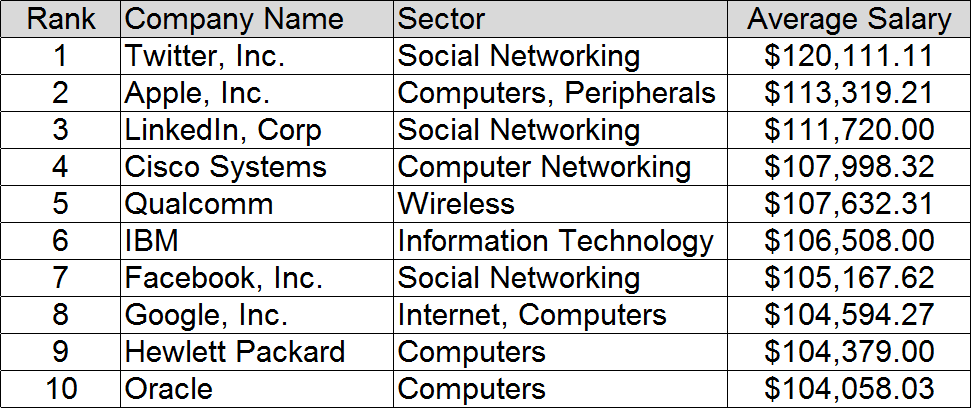
\includegraphics[width=10cm]{figs/toppaytech.png}
\end{center}


\begin{flushright}
{\tiny
http://img59.imageshack.us/img59/802/toppaytech.png
}
\end{flushright}

\end{frame}


%-----------------------    ---------------------------------

\begin{frame}
\frametitle{¿Qué te piden en estos trabajos?}

\begin{itemize}
   \item Estructuras de datos
   \item Algoritmia
   \item Experiencia en programación
   \item Redes de ordenadores
   \item Sistemas operativos
\end{itemize}

\end{frame}


%-----------------------    ---------------------------------

\begin{frame}
\frametitle{Más lecturas}

\begin{itemize}
   \item Hay varios libros sobre este tema, algunos en la biblioteca:
   \begin{itemize}
     \item Cracking the coding interview: 150 programming interview questions and solutions
     \item The Google Interview
     \item Elements of Programming Interviews: The Insiders' Guide
     \item Top 10 coding interview problems asked in Google with solutions: Algorithmic Approach
     \item Are You Smart Enough to Work at Google?: Fiendish Puzzles And Impossible Interview Questions From The World's Top Companies
     \item Get a Job WITHOUT an Interview - Google \& Beyond!: ``We don't mind to lose a good applicant, but definitely not hire a bad applicant.''
     \item The Google Resume: How to Prepare for a Career and Land a Job at Apple, Microsoft, Google, or any Top Tech Company
   \end{itemize}
\end{itemize}

\end{frame}



 % grex
%
%

%%-----------------------------------------------------
%%-----------------------------------------------------
\section{Viéndose con gente...}

%%-----------------------------------------------------
\begin{frame}
\frametitle{Meetup}

\begin{columns}[T]
\begin{column}{.48\textwidth}
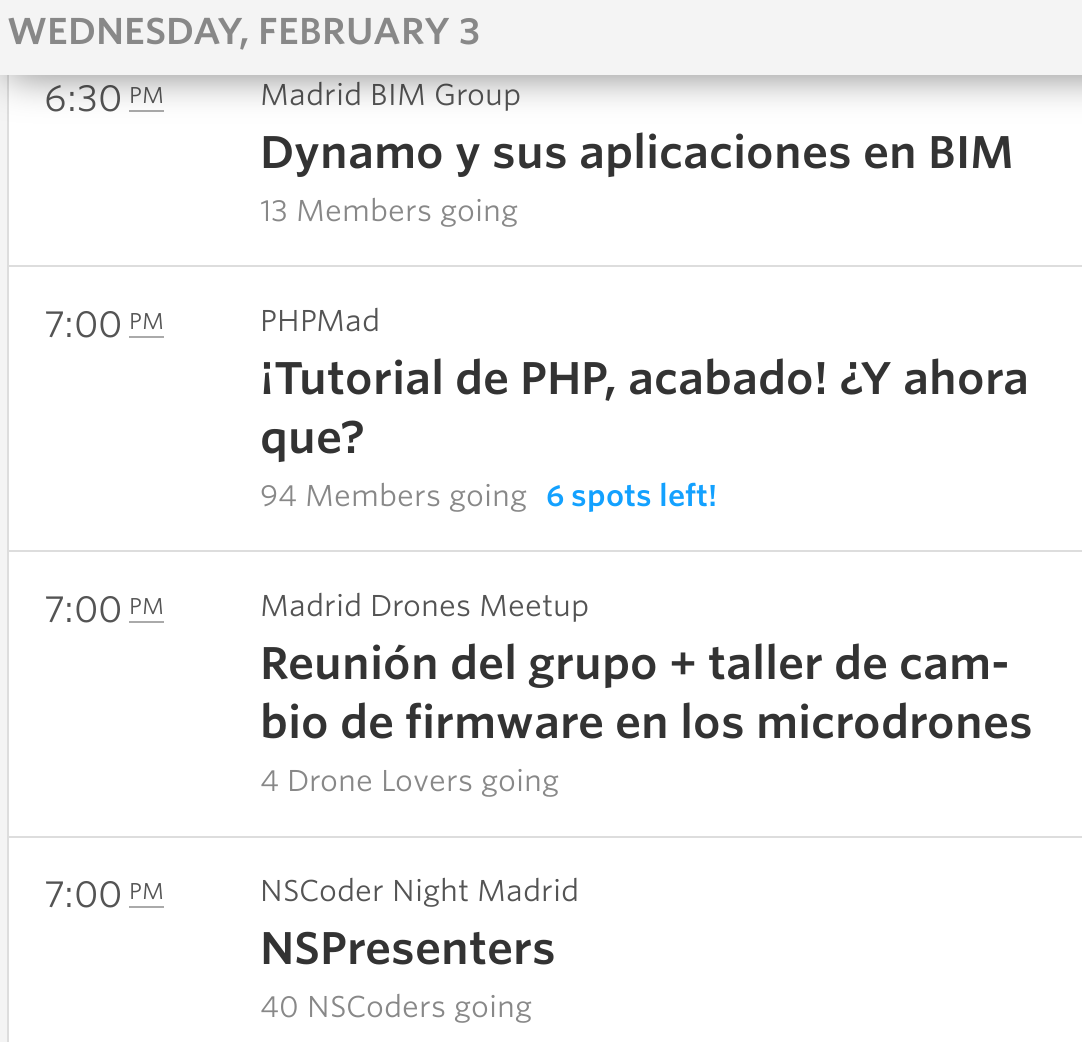
\includegraphics[width=6.5cm]{figs/meetup-calendar}

\begin{flushright}
  {\Large
    \url{http://meetup.com}
  }
\end{flushright}

\end{column}%
\hfill%
\begin{column}{.50\textwidth}
  \begin{flushright}
    
\includegraphics[width=5cm]{figs/meetup-logo}
  \end{flushright}
{\Large
\begin{itemize}
\item Información sobre reuniones cercanas
\item Mucho contenido ténico
\item Y mucho que no
\end{itemize}
}
\end{column}%
\end{columns}

\end{frame}

%%-----------------------------------------------------
\begin{frame}
\frametitle{Grupos}

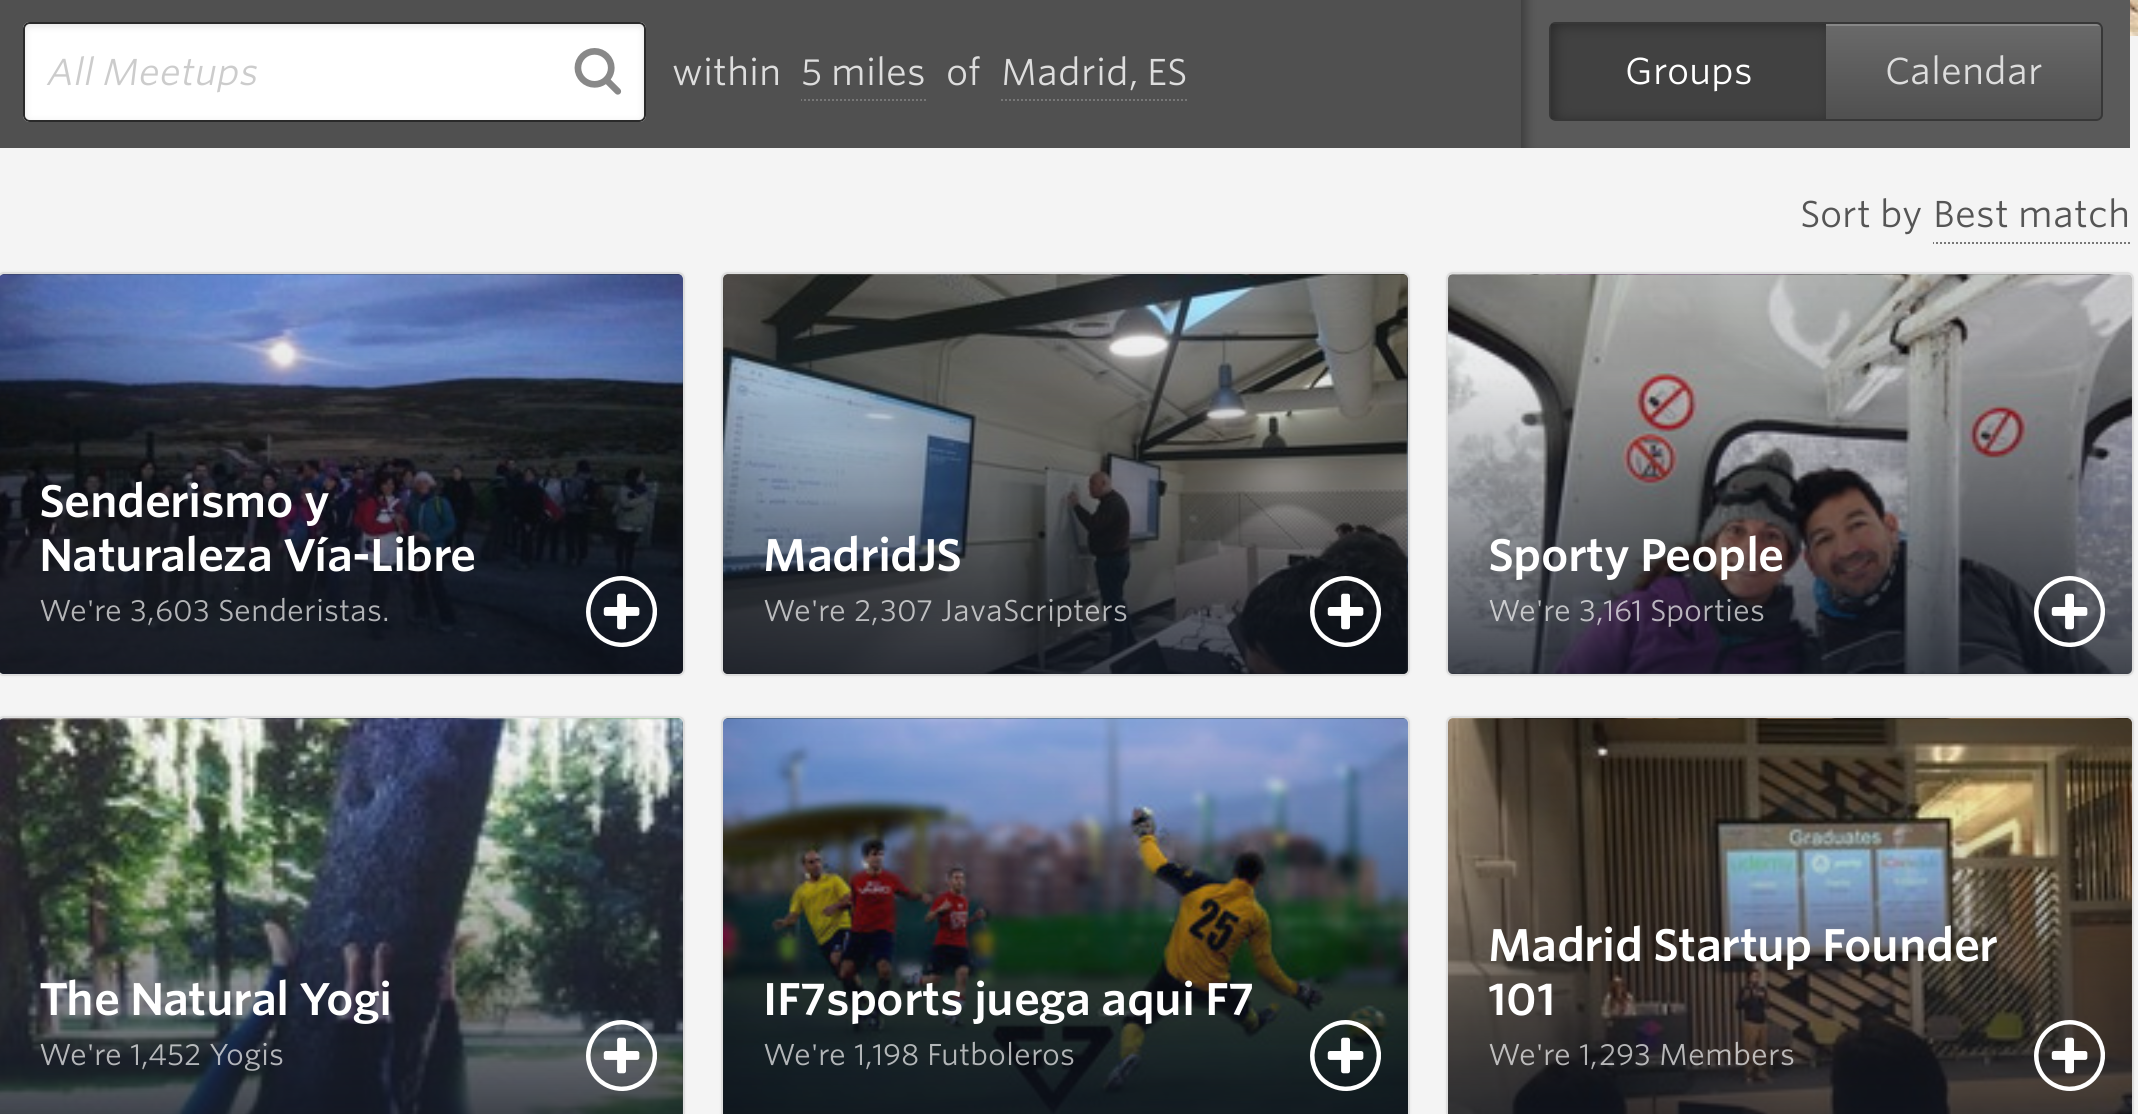
\includegraphics[width=11.5cm]{figs/meetup-near-madrid} 

\end{frame}

%%-----------------------------------------------------
\begin{frame}
\frametitle{Reuniones}

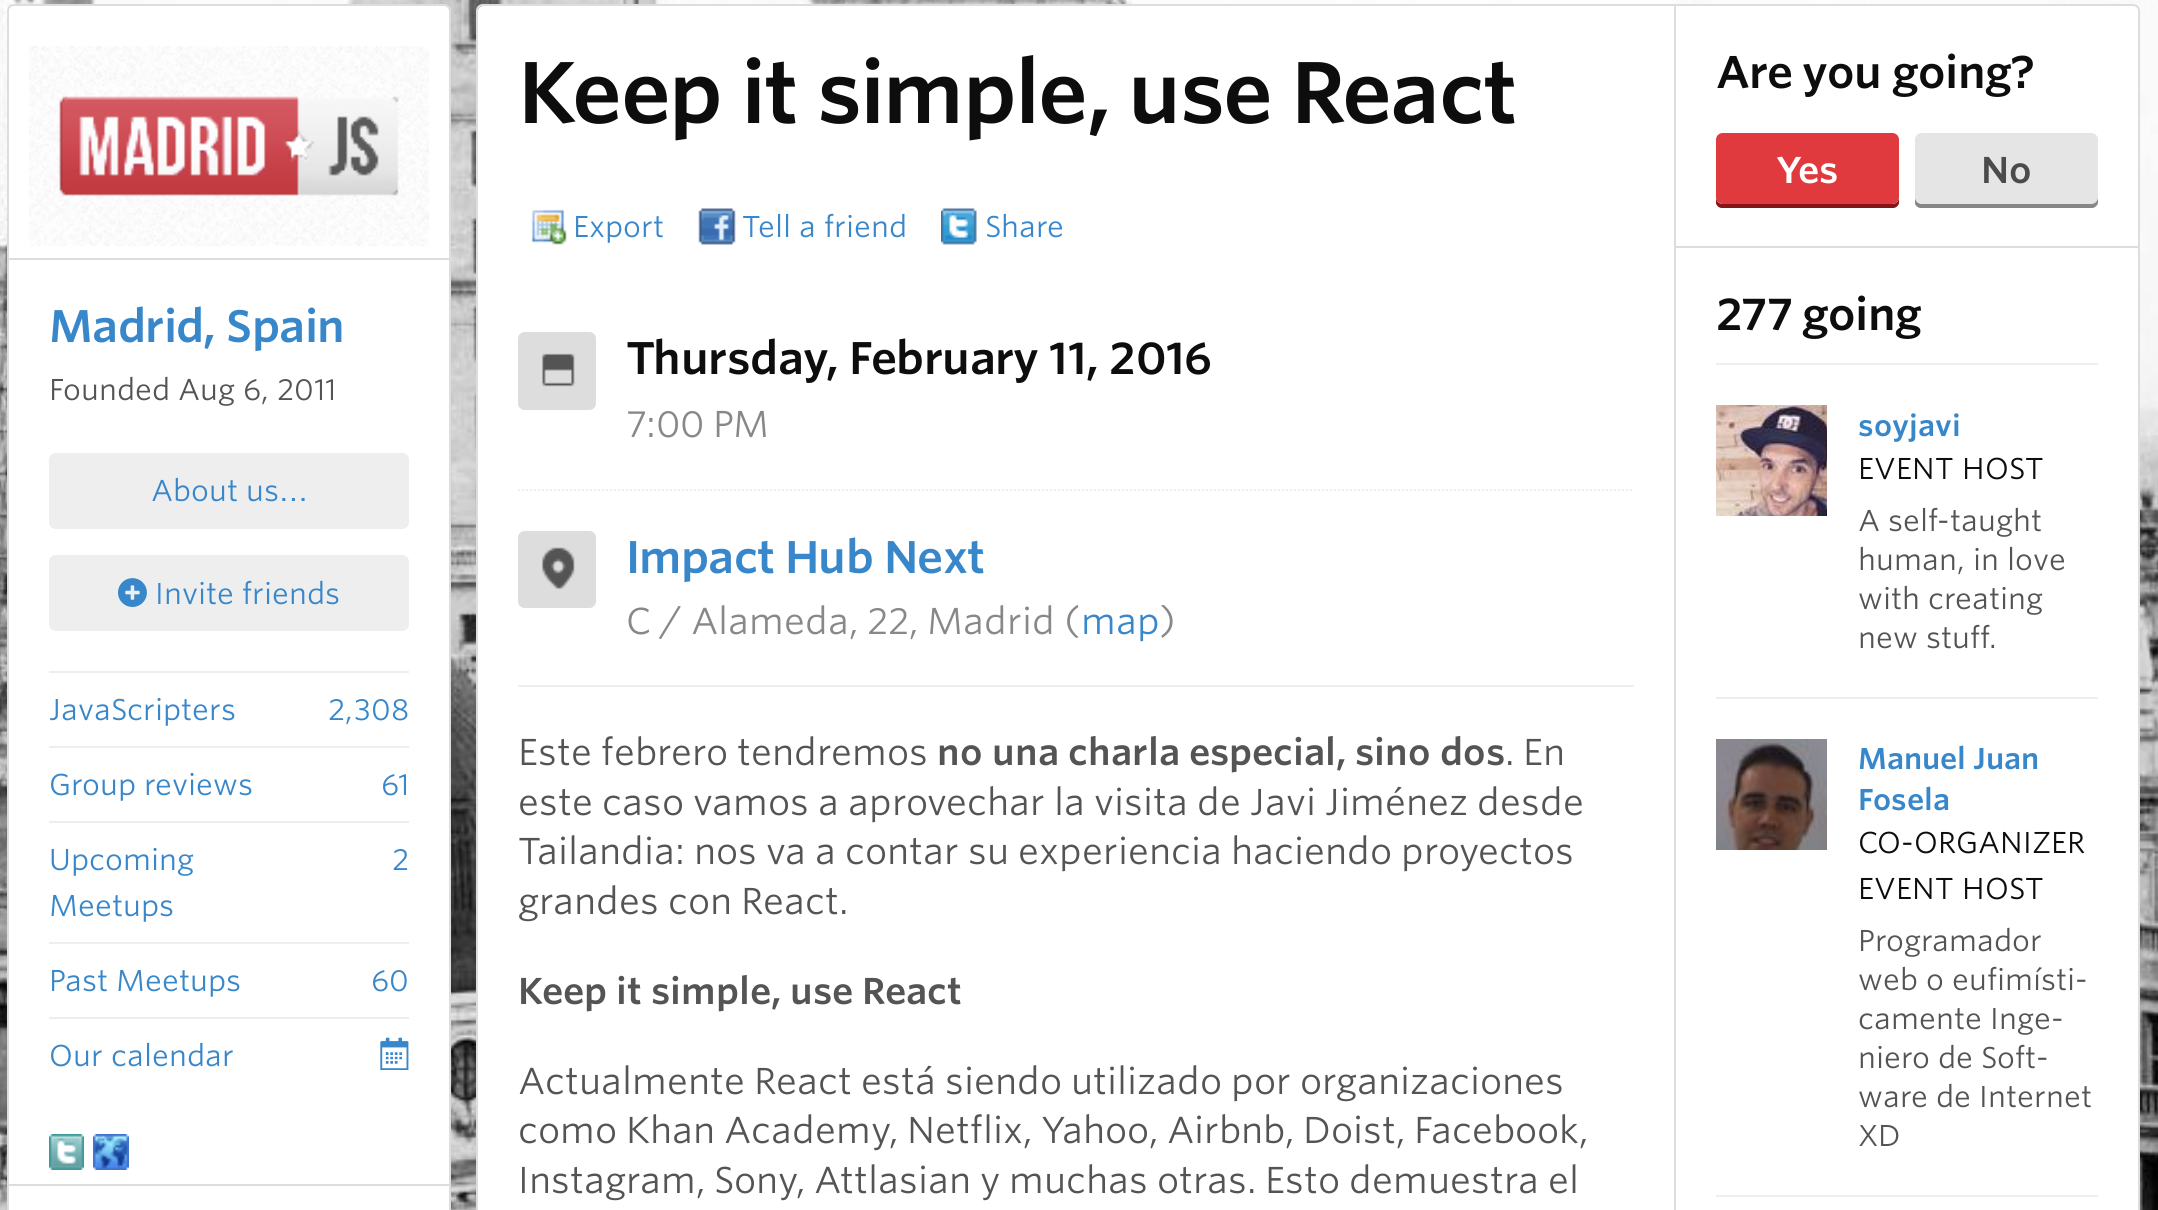
\includegraphics[width=11.5cm]{figs/meetup-meeting} 

\end{frame}






 % jgb
%
%

%%-----------------------------------------------------
%%-----------------------------------------------------
\section{Servidor web en Producción}

%%-----------------------------------------------------
\begin{frame}
\frametitle{Lo que enseñamos en clase}

\begin{columns}[T]
\begin{column}{.48\textwidth}
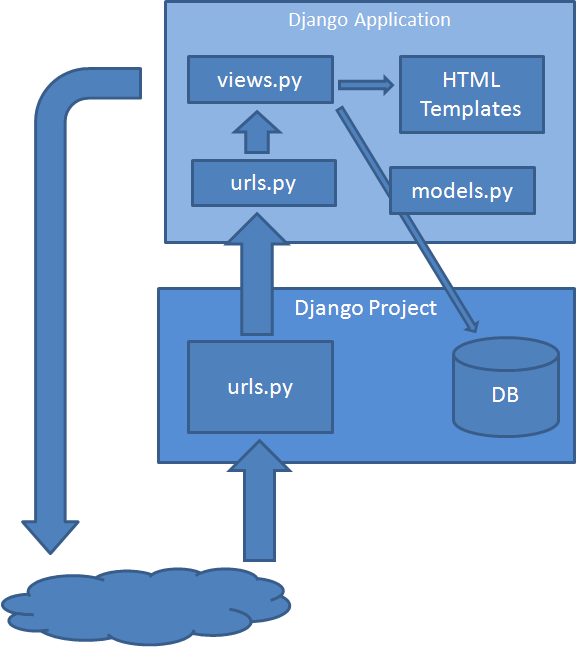
\includegraphics[width=6.5cm]{figs/django}

\begin{flushright}
  {\Large
    \url{http://django-project.com}
  }
\end{flushright}

\end{column}%
\hfill%
\begin{column}{.50\textwidth}
{\Large
\begin{itemize}
  \item Mono-hilo
  \item Mono-tarea
  \item Caché básico
  \item Base de datos limitada (sqlite)
  \item Pensado para páginas dinámicas
  \item Sin planificación
  \item No tiempo real
\end{itemize}
}
\end{column}%
\end{columns}

\end{frame}

%%-----------------------------------------------------
\begin{frame}
\frametitle{Un servidor web en producción}

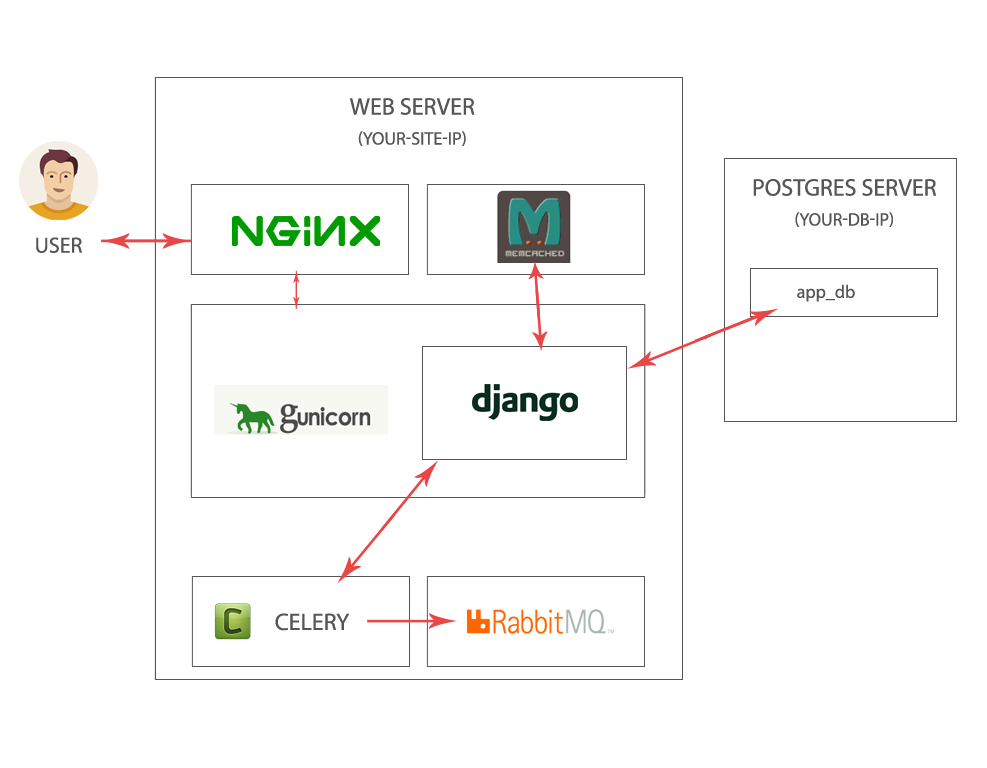
\includegraphics[width=11.5cm]{figs/django-y-mas} 

\end{frame}

%%-----------------------------------------------------
\begin{frame}
\frametitle{Tecnologías}

\begin{itemize}
  \item Django: Framework web
  \item Nginx: Servidor web con balanceo de carga (http://nginx.org/)
  \item Memcached: Caché (http://memcached.org/)
  \item gunicorn: Servidor HTTP (http://gunicorn.org/)
  \item Celery: Tiempo real y planificación de tareas (http://www.celeryproject.org/)
  \item RabbitMQ: Mensajería (https://www.rabbitmq.com/)
  \item PostgreSQL: Base de datos (http://www.postgresql.org/)
\end{itemize}

\end{frame}






 % grex
%
%

%%-----------------------------------------------------
%%-----------------------------------------------------
\usebackgroundtemplate{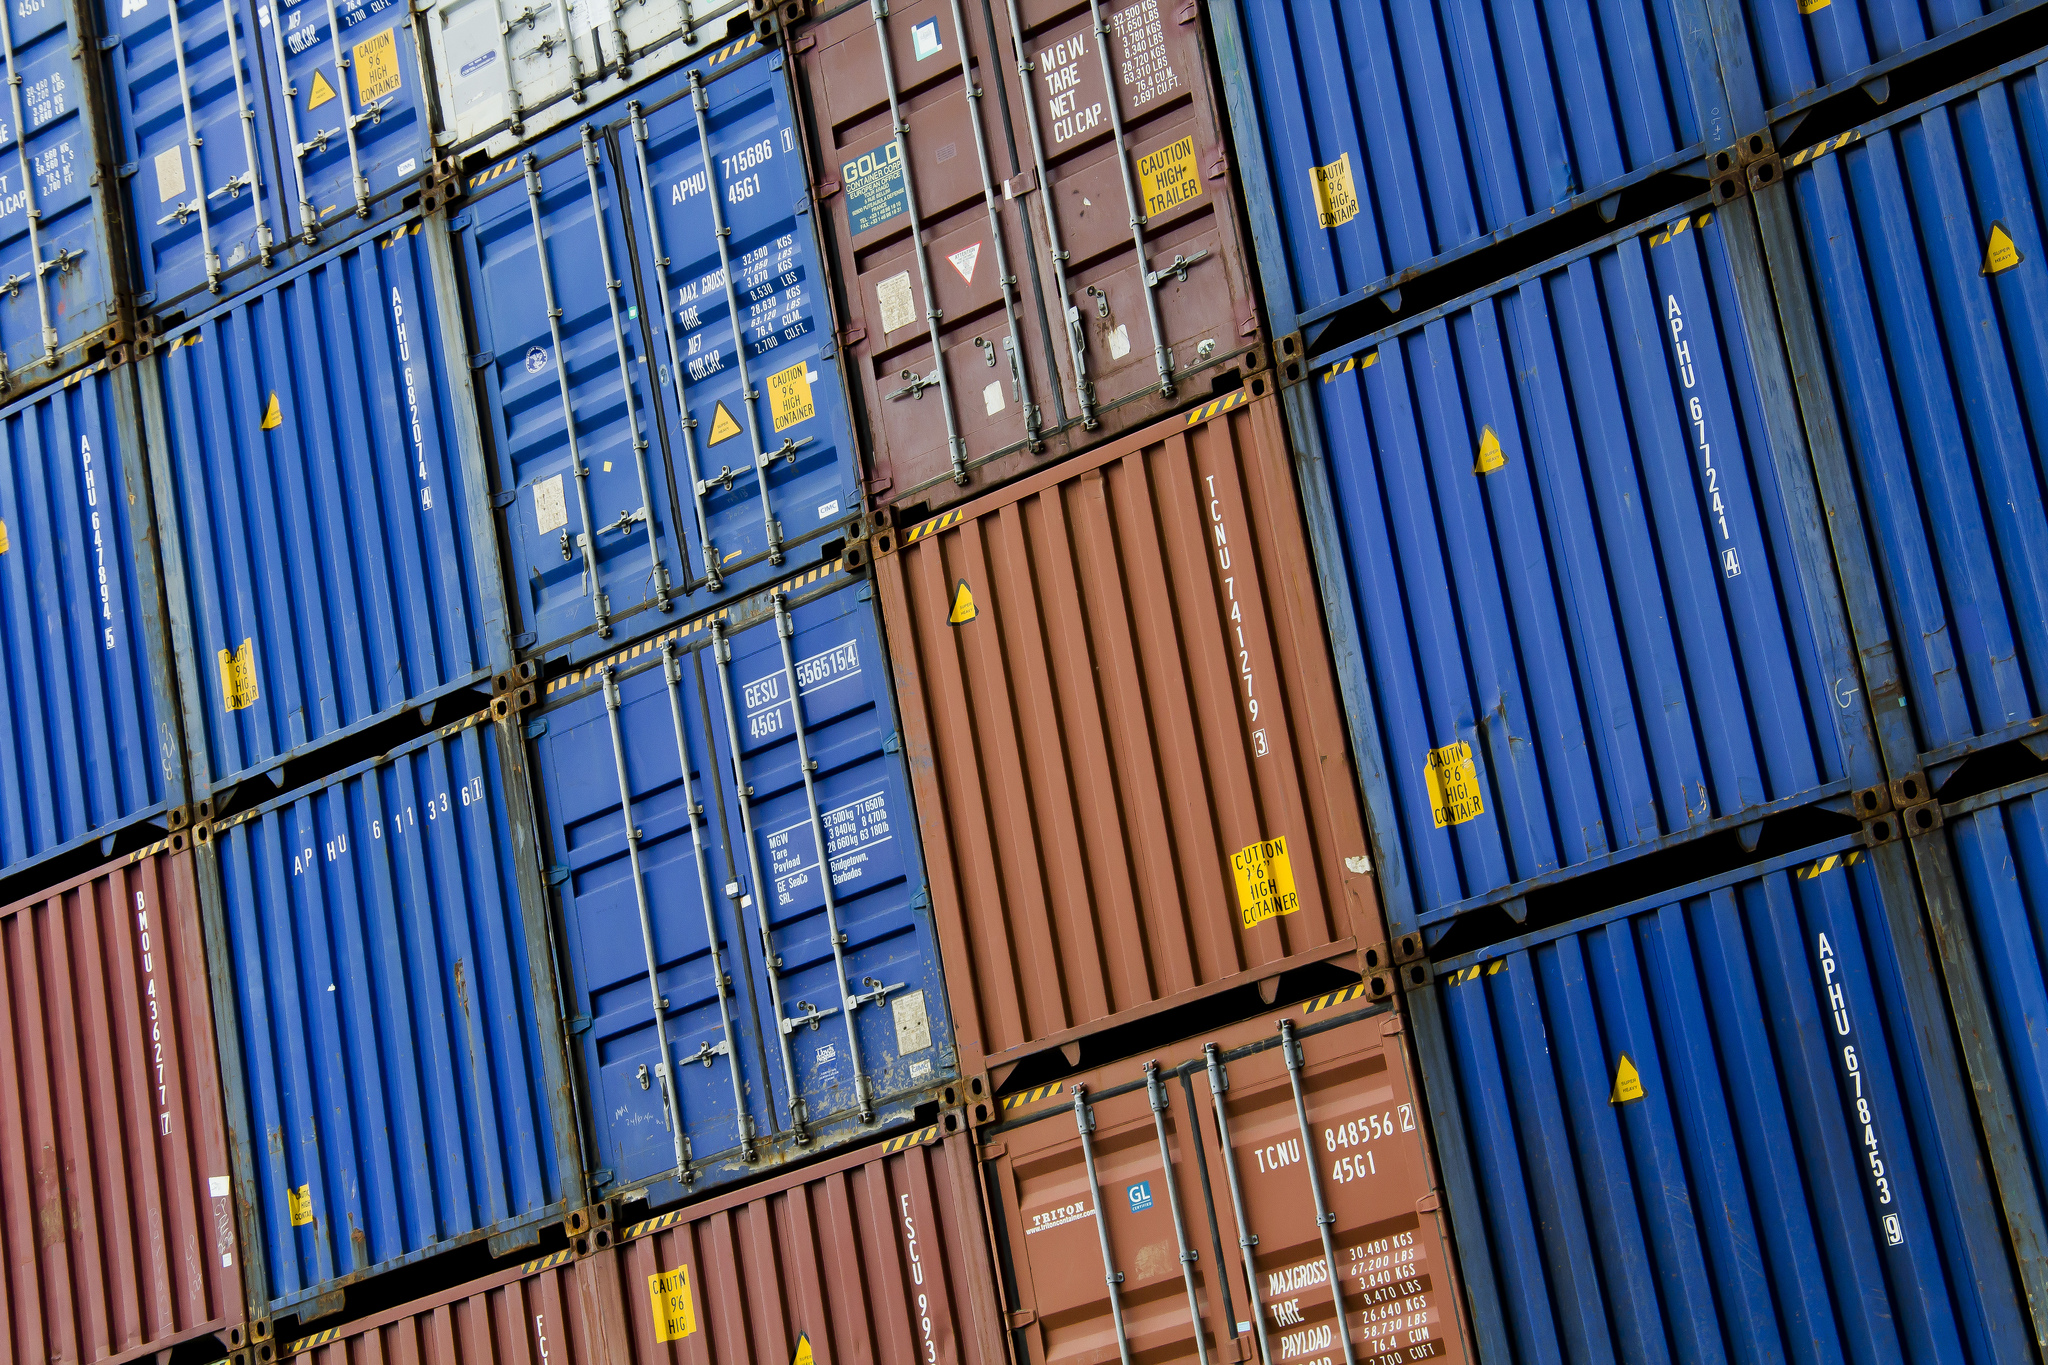
\includegraphics[width=\paperwidth,height=\paperheight]{figs/docker-containers.jpg}}
% Original figure: Flickr, Luke Price, ``Containers, Port of Rotterdam'', CC-by 2.0
% https://www.flickr.com/photos/lukeprice88/9703431992
{\bf
  \textcolor[rgb]{1,1,1}{
    \section{Contenedores por todas partes}
  }
}

\usebackgroundtemplate{}

%%-----------------------------------------------------
\begin{frame}
\frametitle{Contenedores software}

\begin{columns}[T]
\begin{column}{.48\textwidth}
{\Large
  \begin{itemize}
  \item Virtualización sobre sistema operativo
  \item Evolución de la idea de chroot
  \item Aislamiento \\
    (disco, memoria) \\
  \item Gestión de recursos
  \end{itemize}
}
\end{column}%
\hfill%
\begin{column}{.40\textwidth}
{\Large
  \begin{itemize}
  \item Más ligero que máquinas virtuales completas
  \item Mismo kernel \\
    que host \\
  \item Docker, LXC, LXD, \\
    FreeBSD Jail... \\
\end{itemize}
}
\end{column}%
\end{columns}

\end{frame}


%%-----------------------------------------------------
\begin{frame}
\frametitle{Docker (search trend)}

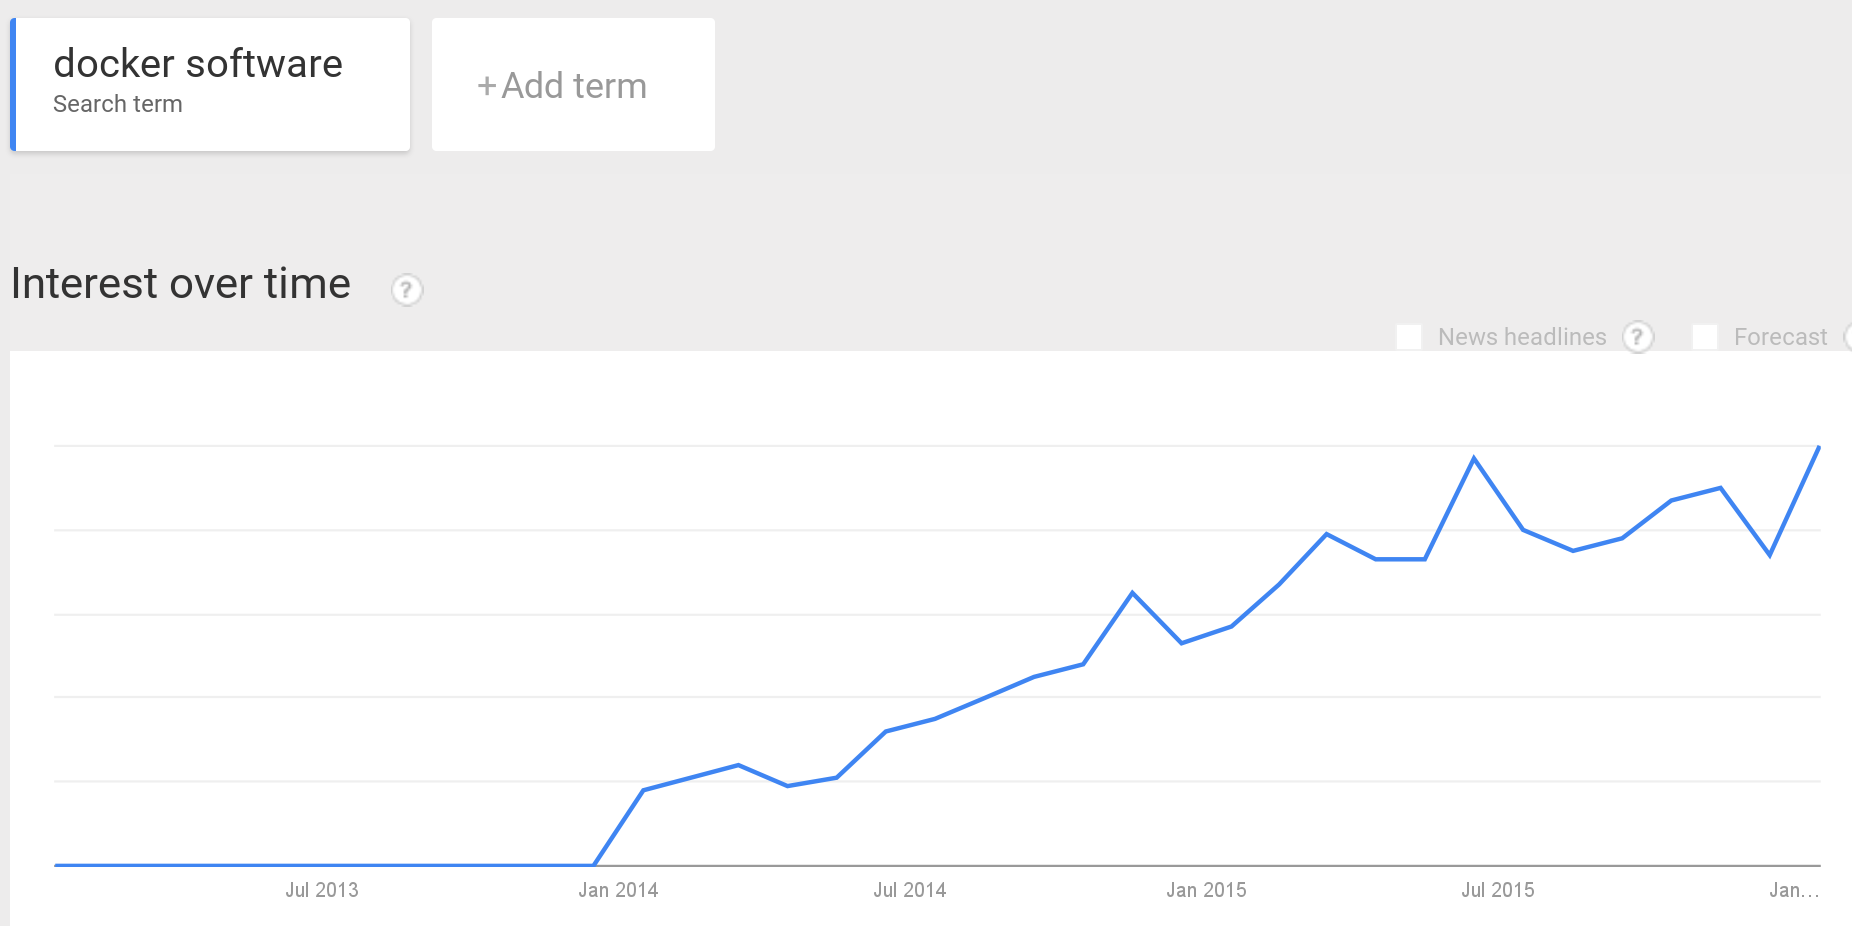
\includegraphics[width=12cm]{figs/docker-trend}


\end{frame}

%%-----------------------------------------------------
\begin{frame}
\frametitle{Docker}


\includegraphics[width=7cm]{figs/docker-logo}

\begin{columns}[T]
\begin{column}{.38\textwidth}

\begin{flushright}
{\Large
  \url{http://docker.com} 

  \vspace{1cm}

  \url{http://hub.docker.com/}
}
\end{flushright}

\end{column}%
\hfill%
\begin{column}{.60\textwidth}
{\Large
\begin{itemize}
\item Automatización del despliegue de aplicaciones en contenedores software
\item Montado sobre cgroups \\ (gestión de recursos), \\
  namespaces \\ (separación de recursos), \\
  sistema de ficheros con unión \\
\end{itemize}
}
\end{column}%
\end{columns}

\end{frame}

%%-----------------------------------------------------
\begin{frame}
\frametitle{Referencias y enlaces}

\begin{flushright}
  Luke Price, ``Containers, Port of Rotterdam'', CC-by 2.0 \\
  \url{https://www.flickr.com/photos/lukeprice88/9703431992} \\
\end{flushright}  

\end{frame}






 % jgb
\include{vm} % jgb
%
%

%%-----------------------------------------------------
%%-----------------------------------------------------
\section{Atom}

%%-----------------------------------------------------
\begin{frame}
\frametitle{Introduciendo Atom}

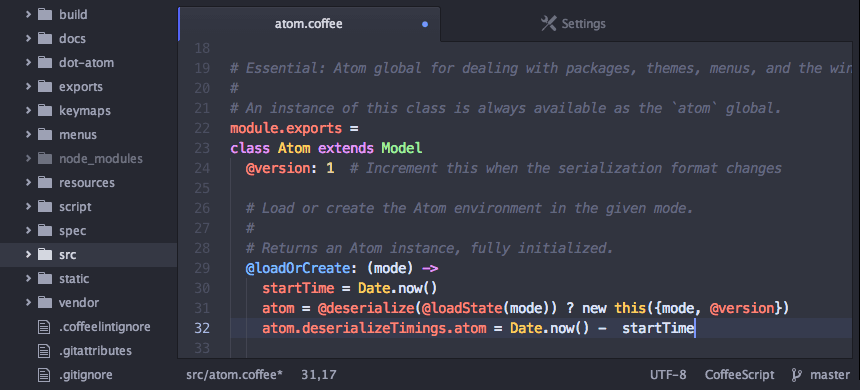
\includegraphics[width=12cm]{figs/atom.png}

\vspace{0.3cm}

  {\Large
    \url{http://atom.io} (Hay paquete Debian)
  }
  
\end{frame}

%%-----------------------------------------------------
\begin{frame}
\frametitle{Características}

\begin{itemize}
  \item Basado HTML, JavaScript, CSS, and Node.js 
  \item Programado en CoffeeScript (compilado a JavaScript)
  \item Autocompletado
  \item Paquetes adicionales
  \item Muchos temas
  \item Configurable
  \item Multiplataforma
  \item ... y es software libre
\end{itemize}

\end{frame}






 % grex
%
%

%%-----------------------------------------------------
%%-----------------------------------------------------
\section{Coffeescript}

%%-----------------------------------------------------
\begin{frame}
\frametitle{The basics}

\begin{columns}[T]
\begin{column}{.48\textwidth}
\begin{center}

\includegraphics[width=3.5cm]{figs/coffeescript}
\end{center}
\begin{flushright}
  {\Large
    \url{coffeescript.org}
  }
\end{flushright}

\end{column}%
\hfill%
\begin{column}{.50\textwidth}
{\Large
\begin{itemize}
  \item Sintaxis más sencilla
  \item Orientado a ser legible
  \item Breve
  \item Indentación
  \item No hay paréntesis
  \item En 2012 fue el 11º lenguage más popular en GitHub
  \item Se puede probar en línea
\end{itemize}
}
\end{column}%
\end{columns}

\end{frame}

%%-----------------------------------------------------
\begin{frame}
\frametitle{¿Cómo funciona?}

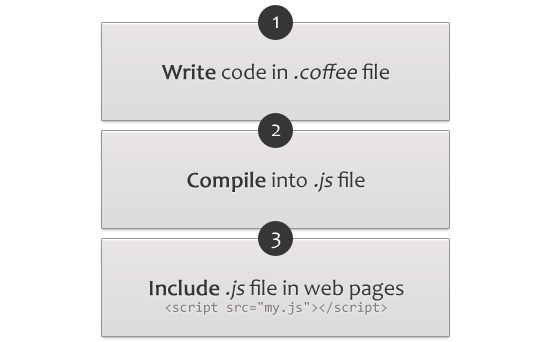
\includegraphics[width=11.5cm]{figs/coffeescript_works.jpg} 
% Imagen sacada de http://sixrevisions.com/javascript/coffeescript-basics/

\end{frame}

%%-----------------------------------------------------
\begin{frame}
\frametitle{Ejemplos}

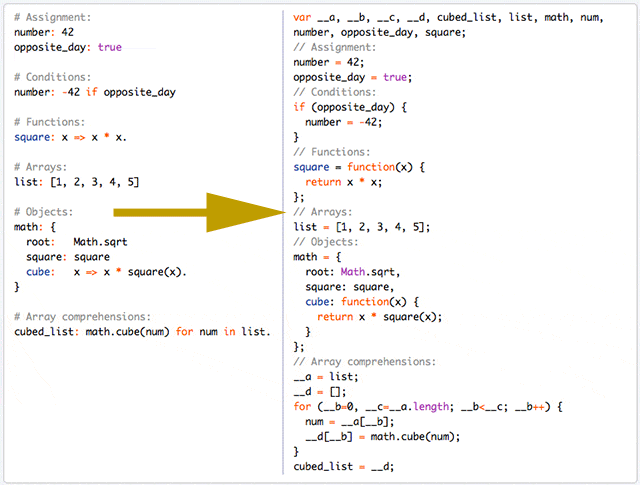
\includegraphics[width=11.5cm]{figs/coffeescript_example.png} 
% Imagen sacada de http://www.rubyinside.com/rails-3-1-adopts-coffeescript-jquery-sass-and-controversy-4669.html


\end{frame}






 % grex

\end{document}
